\documentclass{article}

\usepackage{arxiv}
\usepackage[utf8]{inputenc}
\usepackage[T1]{fontenc}
\usepackage{hyperref}
\usepackage{url}
\usepackage{booktabs}
\usepackage{amsfonts}
\usepackage{amsmath}
\usepackage{amssymb}
\usepackage{nicefrac}
\usepackage{microtype}
\usepackage{graphicx}
\usepackage[numbers]{natbib}
\usepackage{doi}
\usepackage{pgfplots}
\usepackage{tikz}
\usepackage{siunitx}
\usepackage{subcaption}
\usepackage{algorithm}
\usepackage{algpseudocode}
\usepackage{fontawesome5}
\usepackage{placeins}

\usetikzlibrary{arrows.meta, positioning, shapes.geometric, calc, decorations.markings, patterns, fit, backgrounds}
\usepgfplotslibrary{groupplots}
\pgfplotsset{compat=1.18}

\newcommand{\vect}[1]{\mathbf{#1}}
\newcommand{\mat}[1]{\mathbf{#1}}
\newcommand{\R}{\mathbb{R}}
\newcommand{\E}{\mathbb{E}}
\newcommand{\Sph}{\mathbb{S}}
\DeclareMathOperator*{\argmin}{argmin}
\DeclareMathOperator{\logsumexp}{LogSumExp}
\DeclareMathOperator{\logdet}{logdet}
\DeclareMathOperator{\tr}{tr}
\DeclareMathOperator{\Cov}{Cov}
\DeclareMathOperator{\Var}{Var}
\DeclareMathOperator{\Corr}{Corr}
\DeclareMathOperator{\sg}{sg}

\newcommand\figref{Figure~\ref}
\renewcommand\eqref{Equation~\ref}
\newcommand\tabref{Table~\ref}
\newcommand*{\secref}[1]{\hyperref[{#1}]{\S\ref*{#1}}}

\title{What Does Feature Norm Encode in\\
Flat-Space Self-Supervised Learning?}

\author{%
    \href{https://orcid.org/0000-0002-7227-4946}{
\includegraphics[scale=0.06]{orcid.pdf}\hspace{1mm}Shreeyam Kacker} \\
    Department of Aeronautics and Astronautics\\
    MIT\\
    \texttt{shreeyam@mit.edu}
}

\renewcommand{\headeright}{}
\renewcommand{\undertitle}{}
\renewcommand{\shorttitle}{Norm as Confidence in Flat-Space SSL}

\hypersetup{%
    pdftitle={What Does Feature Norm Encode in Flat-Space Self-Supervised Learning?},
    pdfsubject={cs.CV, cs.LG},
    pdfauthor={Shreeyam Kacker},
    pdfkeywords={self-supervised learning, feature norm, out-of-distribution detection, representation geometry}
}

\begin{document}
\maketitle

\begin{abstract}
We investigate a geometric property of self-supervised representations trained
with a flat-Gaussian objective---alignment loss plus a correlation-rate
regularizer and a two-sided variance penalty---and find that the $L_2$ norm of
a learned embedding empirically tracks the model's prediction confidence. On
CIFAR-10, $k$-NN accuracy rises from $44\%$ for low-norm features to $92\%$
for high-norm features; mean feature norm correlates almost perfectly
($r = 0.99$) with distance from the class centroid. When inputs are linearly
mixed with uniform noise, the embedding contracts radially toward the origin,
and pure-noise inputs collapse into a $\sim 12$-dimensional subspace
(vs.\ $\sim 237$ for real images) oriented roughly orthogonal to all class
directions. None of this was trained for: no labels, no confidence
supervision, no out-of-distribution (OOD) examples. By contrast, the publicly
available spherical-SSL model DINOv2 exhibits the \emph{opposite} pattern on
the same stimuli---feature norm \emph{grows} with noise fraction---suggesting
that the phenomenon is specific to the flat-Gaussian geometry rather than a
generic consequence of joint-embedding SSL. We draw connections to MagFace,
energy-based OOD detection, and dimensional collapse, and discuss implications
for using feature norm as a free confidence signal at test time.
\end{abstract}

\noindent\textbf{Keywords:} self-supervised learning, feature norm, out-of-distribution detection, representation geometry

\section{Introduction}
\label{sec:introduction}

Self-supervised learning (SSL) methods based on joint embedding---DINO \citep{caron2021emerging}, DINOv2 \citep{oquab2023dinov2}, BYOL \citep{grill2020byol}, VICReg \citep{bardes2022vicreg}, and more recently SimDINO \citep{wu2025simdino}---learn representations that transfer to downstream tasks without labels. Most such methods $\ell_2$-normalize their output, so the learned features live on a unit hypersphere $\Sph^{d-1}$ and all feature norms are, by construction, equal to one. This choice is standard, well-motivated for contrastive losses, and usually not revisited.

Recent work on coding-rate regularization \citep{yu2020mcr2, wu2025simdino} and variance-covariance regularization \citep{bardes2022vicreg, zbontar2021barlow} makes it possible to train joint-embedding models \emph{without} the final $\ell_2$-normalization, instead constraining the distribution of features to be approximately isotropic Gaussian in $\R^d$. We refer to such models as \emph{flat-space} SSL, in contrast to the spherical-space SSL of DINO. In a flat-space model, feature norms are allowed to vary, so the magnitude $\|\vect{z}\|$ becomes an additional degree of freedom the network can use.

In this paper we ask a simple empirical question: \emph{what does the feature norm of a flat-space SSL model encode?} We train a ResNet-18 \citep{he2016resnet} on CIFAR-10 \citep{krizhevsky2009cifar} with a minimalist flat-Gaussian objective---a cross-view mean-squared alignment loss, a correlation-rate regularizer \citep{ma2007segmentation, wu2025simdino}, and a two-sided variance penalty \citep{schaeffer2024sigreg}---and analyze the geometry of the learned features. The findings are:

\begin{enumerate}
    \item \textbf{Feature norm tracks confidence}. The $k$-nearest-neighbour classification accuracy of a test sample is a strong monotone function of its feature norm: $44\%$ accuracy for the lowest-norm tenth of test samples, $92\%$ for the highest (\secref{sec:experiments}). The Pearson correlation between feature norm and distance from the empirical class centroid is $r = 0.99$.
    \item \textbf{Corruption contracts embeddings radially toward the origin}. Linearly mixing a real image with uniform random noise (mix fraction $\alpha \in [0, 1]$) monotonically reduces the feature norm from its clean value of $\sim 14.8$ to a stable floor of $\sim 11.5$ at $\alpha \ge 0.5$. The direction of the feature also drifts, but the radial contraction dominates.
    \item \textbf{Pure noise collapses onto a low-dimensional subspace orthogonal to the class manifold}. Real-data features are effectively full-rank ($\sim 237$ of $256$ dimensions), while pure-noise features concentrate in a $\sim 12$-dimensional subspace oriented at approximately $80^\circ$ from every class centroid. The encoder has, without supervision, carved out a distinct ``I do not know'' region.
    \item \textbf{The phenomenon does not appear in spherical-SSL models}. Running the same noise-injection experiment on the publicly available DINOv2 \citep{oquab2023dinov2} produces the opposite behaviour: the (unnormalized) CLS-token and patch-pooled feature norms \emph{increase} with noise fraction. Whatever is happening in our model is not a generic property of joint-embedding SSL; it is specific to the flat-Gaussian geometry.
\end{enumerate}

Findings in isolation have precedent. Concurrent work by Draganov et al.~\citep{draganov2025embedding_norms} establishes a norm--accuracy ranking in \emph{cosine-similarity} SSL (SimCLR, SimSiam, BYOL), attributing it to a density-of-updates mechanism on the pre-projection features; CSI \citep{tack2020csi} uses norm as an OOD score on SimCLR. Feature norm as a quality signal is familiar from face recognition \citep{meng2021magface, kim2022adaface}; feature/logit magnitude as an OOD score is the basis of energy-based detectors \citep{liu2020energy}; and dimensional collapse in contrastive SSL has been studied as a failure mode \citep{jing2022dimensional}. Our scope is specifically flat-space SSL---a setting not covered by \citep{draganov2025embedding_norms} and where the norm enters the training objective directly---and our contribution is to characterize the radial-contraction response to continuous input corruption, the low-dimensional pure-noise subspace, and a DINOv2 counterexample showing the sign of the coupling is not automatic.

The paper is organized as follows. \secref{sec:related_work} surveys the three literatures that converge here---flat-space SSL, feature-norm-as-quality, and OOD detection. \secref{sec:method} describes our training objective. \secref{sec:experiments} presents the empirical analysis, including the DINOv2 comparison.

\section{Related Work}
\label{sec:related_work}

\subsection{Joint-Embedding Self-Supervised Learning}

Joint-embedding SSL methods learn representations by aligning features of augmented views of the same image. DINO \citep{caron2021emerging} and its successor DINOv2 \citep{oquab2023dinov2} use a student--teacher framework with cross-entropy over softmax probabilities; BYOL \citep{grill2020byol} uses a stop-gradient predictor; SimCLR \citep{chen2020simclr} uses a contrastive loss with negatives. All of these methods $\ell_2$-normalize the projection-head output, placing features on the unit hypersphere.

A parallel line of work enforces non-collapse via explicit regularization of the feature distribution rather than through the softmax-prototype or contrastive mechanisms. VICReg \citep{bardes2022vicreg} regularizes per-dimension variance and off-diagonal covariance; Barlow Twins \citep{zbontar2021barlow} decorrelates dimensions by penalizing off-diagonals of the cross-correlation matrix; MCR\textsuperscript{2} \citep{yu2020mcr2} maximizes the coding rate \citep{ma2007segmentation} of the representation. Most recently, SimDINO and SimDINOv2 \citep{wu2025simdino} remove the DINO head, softmax, centering, and sharpening entirely, replacing them with a squared-Euclidean alignment loss and a single coding-rate regularizer. SimDINO matches or exceeds DINO/DINOv2 performance with substantially less machinery. Our objective is a close variant of SimDINO adapted for unnormalized features: we use the coding rate on the correlation matrix \citep{kacker2025correlation_rate} rather than the covariance, and we add a two-sided variance penalty (SigReg \citep{schaeffer2024sigreg}) to pin the feature scale.

\subsection{Feature Norm as Confidence in SSL}

The closest prior work to ours is Draganov et al.~\citep{draganov2025embedding_norms}, who argue that in cosine-similarity SSL methods---specifically SimCLR, SimSiam, and BYOL---the unnormalized pre-projection embedding norm encodes a model-confidence signal. Their mechanism is density-based: frequently observed patterns receive more gradient updates and their embeddings grow larger, so typical samples end up with higher norms than atypical ones. They demonstrate the norm--accuracy coupling on several benchmarks and report that OOD inputs receive smaller norms. We share the headline finding in the norm-accuracy ranking, but our setting and scope differ. Their analysis covers \emph{spherical} SSL models whose training objective operates on $\ell_2$-normalized features; the norm they study is a by-product of the penultimate layer. We instead study \emph{flat-space} SSL, where the embedding norm enters the loss directly through the variance regularizer, and we characterize how the norm responds to continuous input corruption (\secref{sec:noise}) and where pure-noise inputs are placed in feature space (\secref{sec:noise_subspace})---neither of which is examined by Draganov et al. Our DINOv2 comparison (\secref{sec:dinov2}) also shows that the direction of the coupling is not automatic, even within spherical-SSL.

CSI \citep{tack2020csi} uses $\|\vect{z}\| \cdot \cos(\vect{z}, \vect{z}_\text{nn})$ as an OOD score on SimCLR features, exploiting the tendency of the contrastive objective to inflate in-distribution norms. CSI is a detection-time score built on top of an off-the-shelf contrastive model; our focus is the representation-level geometry itself, in a non-contrastive flat-space setting, without any labeled OOD data to calibrate against.

\subsection{Feature Norm as a Quality Signal}

In face recognition, several works have observed that the magnitude of a learned face embedding correlates with image quality. NormFace \citep{wang2017normface} studied the effect of $\ell_2$ normalization on softmax classifiers. MagFace \citep{meng2021magface} explicitly engineered a loss that makes the feature magnitude correlate with face image quality: low-quality faces (occlusion, blur) are placed near the origin, high-quality frontal faces far from it. AdaFace \citep{kim2022adaface} builds on this idea with a margin that adapts to the norm. Crucially, these works \emph{design for} the norm--quality coupling; they assume that if the loss is structured correctly, useful magnitude information will emerge. Our finding sits in the same conceptual space but arises without any explicit quality signal: the coupling emerges from the flat-Gaussian geometry alone.

\subsection{Energy-Based and Feature-Norm OOD Detection}

A separate literature uses norm-like quantities at test time to distinguish in-distribution from out-of-distribution inputs. Energy-based OOD \citep{liu2020energy} uses $-\logsumexp(\text{logits})$ as an OOD score, which reduces to a norm-like quantity when the classifier head is approximately linear. Mahalanobis-based OOD \citep{lee2018mahalanobis} uses class-conditional feature distributions. ViM \citep{wang2022vim} explicitly combines feature norm with softmax residual. SSD \citep{sehwag2021ssd} uses SimCLR features for OOD detection without labels. These methods typically assume a classifier has been trained and study the resulting feature geometry; our setting is purely self-supervised, and the OOD behavior is a consequence of the representation learning rather than an add-on.

\subsection{Representation Geometry and Dimensional Collapse}

Jing et al.~\citep{jing2022dimensional} study \emph{dimensional collapse} in contrastive SSL, where the learned features occupy a lower-dimensional subspace than the ambient space, usually characterized as a failure mode. Our observation that pure-noise features collapse to a low-dimensional subspace is closely related, but with a different interpretation: the collapse is \emph{selective}. In-distribution features span the full representation space; out-of-distribution inputs are the ones that collapse. This is the intended behavior of an OOD-aware representation, not a pathology.

Several works examine what is encoded in the radial and angular components of learned features \citep{wang2020hypersphere, wang2017normface}. Wang \& Isola \citep{wang2020hypersphere} decompose contrastive objectives into alignment (low angular spread within class) and uniformity (high angular spread across classes); our flat-space setting adds a radial degree of freedom that their framework cannot directly express.

\subsection{Summary of Position}

The literatures above---flat-space SSL, norm-as-confidence in cosine SSL \citep{draganov2025embedding_norms, tack2020csi}, face-recognition norm quality signals, OOD detection, and representation collapse---converge on our finding but have not previously been assembled for flat-space SSL. Draganov et al.~establish the norm-accuracy ranking for spherical SSL; we show the same ranking holds without $\ell_2$ normalization, and go further by characterizing the continuous noise-corruption response and the low-dimensional pure-noise subspace. The face-recognition community designs for norm--quality coupling; we show it emerges for free. The OOD community uses feature norm as a post-hoc detector; we show the detector is built in at representation-learning time. The SSL community has extensive work on avoiding representation collapse; we show that one kind of collapse (for OOD inputs) is a feature, not a bug, under the right geometry.

\section{Method}
\label{sec:method}

Our goal is to learn an encoder $f_\theta : \mathcal{X} \to \R^d$ such that features $\vect{z} = f_\theta(x) \in \R^d$ (i) are view-invariant (two augmentations of the same image produce similar features), (ii) have approximately unit variance along each coordinate, and (iii) have approximately uncorrelated coordinates---i.e., the batch feature distribution approximates $\mathcal{N}(\vect{0}, \mat{I})$. We do not $\ell_2$-normalize the output.

\subsection{Architecture}

The encoder is a standard backbone (ResNet-18 \citep{he2016resnet} in our experiments, with the $7\times 7$ stride-2 stem replaced by a $3\times 3$ stride-1 conv and the initial maxpool removed, as is standard for CIFAR-scale inputs) followed by a three-layer MLP projection head:
\begin{equation}
    f_\theta(x) = h \circ g(x), \qquad h : \R^{d_\text{emb}} \to \R^d,
\end{equation}
where $g$ produces a $d_\text{emb}$-dimensional feature ($d_\text{emb} = 512$ for ResNet-18) and $h$ is Linear--BN--GELU--Linear--BN--GELU--Linear. Unlike DINO \citep{caron2021emerging}, there is no final $\ell_2$ normalization and no weight-normalized prototype layer: the output $\vect{z} \in \R^d$ with $d = 256$ is the feature we study. A teacher network $f_{\bar{\theta}}$ is maintained as an exponential moving average of the student with cosine schedule from $\alpha_0 = 0.99$ to $1$.

\subsection{Loss}

For each input image $x$ we generate two augmented views $v_1, v_2$ (random resized crop, horizontal flip, color jitter, grayscale) and compute student features $\vect{s}_i = f_\theta(v_i)$ and teacher features $\vect{t}_i = f_{\bar\theta}(v_i)$. The total loss combines three terms.

\paragraph{Cross-view alignment.} A squared-Euclidean loss between student features on one view and stop-gradient teacher features on the other:
\begin{equation}
    \mathcal{L}_\text{align} = \tfrac{1}{2}\bigl(\|\vect{s}_1 - \sg(\vect{t}_2)\|^2 + \|\vect{s}_2 - \sg(\vect{t}_1)\|^2\bigr).
\end{equation}
This is the minimalist alignment objective of SimDINO \citep{wu2025simdino}, differing from the original DINO cross-entropy in dropping the softmax, centering, sharpening, and high-dimensional prototype head.

\paragraph{Correlation-rate expansion.} Left to itself, $\mathcal{L}_\text{align}$ admits the trivial optimum $f_\theta \equiv \vect{c}$ (collapse). To prevent collapse we maximize the coding rate \citep{ma2007segmentation, yu2020mcr2} of the batch feature covariance. However, coding rate on the raw covariance is scale-sensitive: as features grow in magnitude, the coding rate grows unboundedly, destabilizing training \citep{kacker2025correlation_rate}. We therefore use the coding rate of the \emph{correlation} matrix. Let $\mat{Z} \in \R^{n \times d}$ be the stacked batch features and $\hat{\mat{Z}} = \mat{Z} \oslash \sigma(\mat{Z})$ the per-dimension-standardized version. The correlation rate is
\begin{equation}
\label{eq:corr_rate}
    R_\varepsilon(\hat{\mat{Z}}) = \tfrac{1}{2}\logdet\!\left(\mat{I}_d + \tfrac{d}{n \varepsilon^2}\, \hat{\mat{Z}}^\top \hat{\mat{Z}}\right),
\end{equation}
which is scale-invariant: multiplying $\mat{Z}$ by any positive constant leaves $\hat{\mat{Z}}$ and hence $R_\varepsilon$ unchanged. The correlation-rate term in the loss is $-\gamma R_\varepsilon(\hat{\mat{Z}})$, with coefficient $\gamma > 0$.

\paragraph{Two-sided variance regularization (SigReg).} Because $R_\varepsilon$ is scale-invariant, nothing in the loss so far anchors the feature scale. We add a two-sided penalty on the per-dimension standard deviation, pinning it to one on both sides \citep{schaeffer2024sigreg}:
\begin{equation}
    \mathcal{L}_\text{sig} = \frac{1}{d} \sum_{j=1}^{d} \bigl(\sigma_j(\mat{Z}) - 1\bigr)^2,
\end{equation}
where $\sigma_j(\mat{Z})$ is the sample standard deviation of feature dimension $j$ across the batch. Note this differs from the ReLU hinge $\max(0, 1 - \sigma_j)$ used in VICReg \citep{bardes2022vicreg}: VICReg's hinge vanishes once $\sigma_j \ge 1$, leaving the feature magnitude unbounded above, whereas $\mathcal{L}_\text{sig}$ actively constrains $\sigma_j$ from both directions.

\paragraph{Total loss.}
\begin{equation}
\label{eq:loss}
    \mathcal{L} = \mathcal{L}_\text{align} + w_\text{sig}\, \mathcal{L}_\text{sig} - \gamma\, R_\varepsilon(\hat{\mat{Z}}),
\end{equation}
with $w_\text{sig} = 1$, $\gamma = 10^{-3}$, and $\varepsilon = 0.5$ in all experiments below. The three coefficients were selected on a preliminary sweep (reported in \secref{sec:experiments}); accuracy is essentially insensitive to $\varepsilon \in [0.1, 1.0]$ and $\gamma \in [3 \cdot 10^{-4}, 3 \cdot 10^{-3}]$, and weakly sensitive to $w_\text{sig}$.

\subsection{Connection to Covariance KL}
\label{sec:covkl}

The objective \eqref{eq:loss} separates scale (via $\mathcal{L}_\text{sig}$) from correlation structure (via $R_\varepsilon$). It is instructive to compare this split against a single basis-free term that captures both at once: the KL divergence of the batch-feature second-order moment to $\mathcal{N}(\vect{0}, \mat{I}_d)$. Let $\mat{C} = \tfrac{1}{n}\tilde{\mat{Z}}^\top \tilde{\mat{Z}}$ be the batch covariance of centered features, with a small shrinkage $\mat{C}_\rho = (1-\rho)\mat{C} + \rho \mat{I}$ for numerical stability. The covariance-KL objective is
\begin{equation}
\label{eq:covkl}
    \mathcal{L}_\text{covKL} \;=\; \tfrac{1}{2}\Bigl(\tr(\mat{C}_\rho) \;-\; \logdet(\mat{C}_\rho) \;-\; d\Bigr)
    \;=\; \mathrm{KL}\!\left(\mathcal{N}(\vect{0}, \mat{C}_\rho) \,\big\|\, \mathcal{N}(\vect{0}, \mat{I}_d)\right).
\end{equation}
Writing $\mat{C} = \mat{D}^{1/2}\mat{R}\mat{D}^{1/2}$ with $\mat{D} = \diag(\sigma_1^2, \dots, \sigma_d^2)$ and $\mat{R}$ the correlation matrix, the scale and structure pieces decompose cleanly:
\begin{equation}
\label{eq:covkl_decomp}
    \tr(\mat{C}) - \logdet(\mat{C}) - d
    \;=\; \underbrace{\sum_{j=1}^{d}\bigl(\sigma_j^2 - 2\log\sigma_j - 1\bigr)}_{\text{diagonal (scale)}} \;-\; \underbrace{\logdet(\mat{R})}_{\text{off-diagonal (decorrelation)}}.
\end{equation}

Our current objective~\eqref{eq:loss} is an \emph{approximation} to each side of this decomposition. Two local discrepancies and two global ones are worth noting.

\paragraph{Scale term: $(\sigma_j - 1)^2$ vs.~$\sigma_j^2 - 2\log\sigma_j - 1$.}
Near $\sigma_j = 1$ the two agree at leading order: a Taylor expansion gives $\sigma_j^2 - 2\log\sigma_j - 1 = 2(\sigma_j - 1)^2 + O\!\bigl((\sigma_j - 1)^3\bigr)$, so $\mathcal{L}_\text{sig}$ is our $(\sigma_j-1)^2$ up to a factor of two. They differ asymptotically: the KL form has a $-\log\sigma_j$ barrier that diverges as $\sigma_j \to 0$, providing a stronger repulsion from per-dimension collapse, and grows sub-quadratically (rather than quadratically) as $\sigma_j \to \infty$, which is less aggressive on directions that want variance slightly above one.

\paragraph{Structure term: $\tfrac{1}{2}\logdet\!\bigl(\mat{I}_d + (d/\varepsilon^2)\mat{R}\bigr)$ vs.~$-\logdet\mat{R}$.}
The correlation-rate expansion inherits its form from coding rate~\citep{yu2020mcr2, wu2025simdino}: the $\mat{I}_d + (d/\varepsilon^2)\mat{R}$ regularization was originally motivated by an additive-noise rate-distortion bound, not as a Gaussian match. It is bounded even as $\mat{R}$ becomes singular: if $\lambda_i(\mat{R}) \to 0$, the corresponding factor $1 + (d/\varepsilon^2)\lambda_i \to 1$ is finite, so the gradient resisting near-singular directions is $O(d/\varepsilon^2)$---large but bounded. In contrast, $-\logdet\mat{R}$ diverges as $\lambda_i \to 0^+$, giving an unbounded barrier against directional collapse. Both have an optimum at $\mat{R} = \mat{I}$ under the constraint $\tr(\mat{R}) = d$, but their off-optimum shapes differ: the coding-rate form is a soft expansion pressure, while $-\logdet$ is a hard anti-collapse barrier.

\paragraph{Global behavior.}
$\mathcal{L}_\text{covKL}$ has a unique minimum at $\mat{C} = \mat{I}_d$, whereas a coding-rate expansion has \emph{no minimum}---its gradient monotonically rewards spread, so the scale must be anchored by a separate term (as we do with $\mathcal{L}_\text{sig}$). This separation has a practical cost: $R_\varepsilon$ operates on standardized features and is therefore blind to the scale the rest of the loss is fighting over, forcing $\mathcal{L}_\text{sig}$ to clean up afterward. The covariance-KL form conflates the two in the natural way: $\tr(\mat{C})$ alone pushes scale down, $-\logdet(\mat{C})$ alone pushes spread up, and equilibrium is at $\mat{C} = \mat{I}$.

We report experiments with the decomposed objective in~\eqref{eq:loss} for continuity with the correlation-rate literature and because the geometric findings of~\secref{sec:experiments} do not depend sensitively on the exact scale term. A clean covariance-KL ablation---replacing $R_\varepsilon - w_\text{sig}\mathcal{L}_\text{sig}$ with a single $\mathcal{L}_\text{covKL}$ term plus an explicit mean penalty $\lambda_\mu \|\bar{\vect{z}}\|^2$---is a natural next step; we leave a systematic comparison to future work.

\subsection{Rationale for the Three Terms}

The three terms play distinct geometric roles:
\begin{itemize}
    \item $\mathcal{L}_\text{align}$ pulls features of different views of the same image together (\emph{alignment}).
    \item $R_\varepsilon$, operating on the correlation matrix, pushes the off-diagonal entries of the correlation toward zero, which makes the batch feature distribution factorize across dimensions (\emph{decorrelation}).
    \item $\mathcal{L}_\text{sig}$ pins the per-dimension scale to one (\emph{variance control}).
\end{itemize}
At convergence, the batch features approximate $\mathcal{N}(\vect{0}, \mat{I}_d)$---zero mean by the symmetry of the optimization, unit per-dimension variance by $\mathcal{L}_\text{sig}$, uncorrelated dimensions by $R_\varepsilon$. The per-sample position within this distribution is unconstrained beyond alignment with the teacher, and it is in this residual freedom---particularly the radial coordinate---that the confidence-like structure we document in \secref{sec:experiments} emerges.

\section{Experiments}
\label{sec:experiments}

We train a ResNet-18 with the objective of \eqref{eq:loss} on CIFAR-10 for 100 epochs at batch size $512$, with AdamW \citep{loshchilov2017adamw} at learning rate $10^{-3}$ and cosine decay, $\alpha_0 = 0.99$ for the EMA teacher, and $w_\text{sig} = 1$, $\gamma = 10^{-3}$, $\varepsilon = 0.5$ as described in \secref{sec:method}. The projection head output dimension is $d = 256$. Evaluations are performed on the CIFAR-10 validation set using $k$-nearest-neighbour classification with $k = 20$ over $\ell_2$-normalized features; linear-probe accuracies are qualitatively consistent.

Under these settings the model reaches $k$-NN accuracy $77.3\%$ at epoch $100$ (compared to $67.8\%$ for a smaller ConvNet under the same objective; $75.1\%$ on the subset of $10{,}000$ validation images used for geometric analysis below). The absolute number is modest---this is a short training run with only two views and limited augmentation---but the \emph{geometry} of the learned features is what we analyze below.

\subsection{Feature Geometry}
\label{sec:geometry}

We extract the projection-head output for all $10{,}000$ validation images and compute summary statistics of the resulting $10{,}000 \times 256$ matrix $\mat{Z}$.

\paragraph{Per-dimension marginals.} The empirical mean along each dimension is $\mu = -0.008 \pm 0.171$ (mean $\pm$ standard deviation across dimensions) and the variance is $\sigma_j^2 = 0.889 \pm 0.021$---close to unit variance per dimension, with very small spread across dimensions. The mean absolute off-diagonal correlation is $0.013$ with a maximum of $0.069$: dimensions are decorrelated to well within typical significance thresholds.

\paragraph{Norm distribution.} The feature norm distribution has $\E\|\vect{z}\| = 15.21$, $\text{std}\|\vect{z}\| = 1.93$. If the features were exactly $\mathcal{N}(\vect{0}, \mat{I}_{256})$, the norm would follow a $\chi_{256}$ distribution with mean $15.98$ and standard deviation $0.71$. The empirical mean norm matches closely ($95\%$ of the theoretical value), but the empirical standard deviation is roughly three times larger---the distribution is fatter-tailed than a true Gaussian's. This extra radial spread is the signature we study in the rest of this section: it is not an artifact of imperfect training, but a load-bearing degree of freedom the encoder uses.

\subsection{Feature Norm and Prediction Confidence}
\label{sec:norm_confidence}

We divide the validation set into deciles by feature norm and measure $k$-NN accuracy within each decile (\figref{fig:norm_vs_acc}).

\begin{figure}[t]
    \centering
    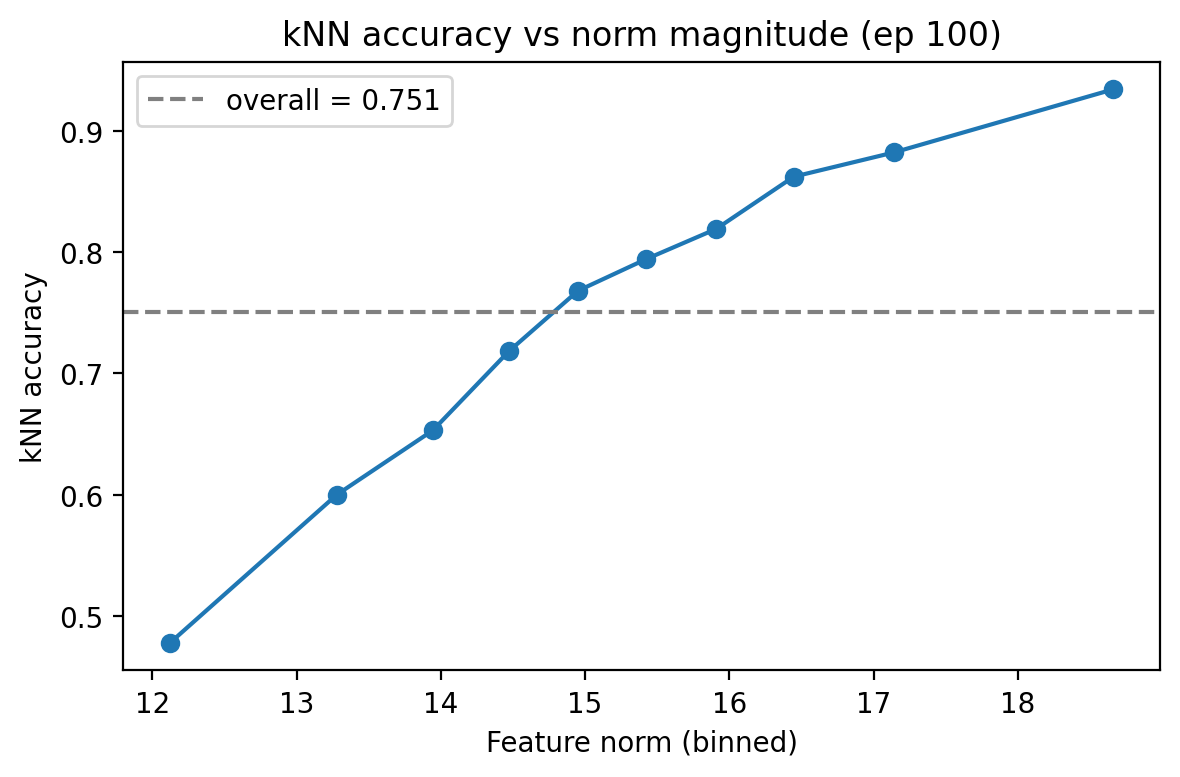
\includegraphics[width=0.52\linewidth]{figures/norm_vs_accuracy_ep100.png}
    \caption{$k$-NN accuracy on CIFAR-10 validation conditioned on feature-norm decile. Accuracy rises from $43.6\%$ in the lowest-norm decile to $91.8\%$ in the highest. Horizontal line: overall accuracy ($73.4\%$ at the epoch shown).}
    \label{fig:norm_vs_acc}
\end{figure}

Accuracy rises monotonically from $43.6\%$ in the lowest-norm decile (features with $\|\vect{z}\| \approx 12$) to $91.8\%$ in the highest (features with $\|\vect{z}\| \approx 19$). Without ever being trained to produce confidence scores, the encoder's feature norm provides a ranking of test samples that is strongly predictive of classification accuracy.

\paragraph{Relation to class structure.} We computed the Pearson correlation between $\|\vect{z}_i\|$ and several candidate explanatory variables (\tabref{tab:correlations}). Distance from the empirical class centroid is almost a perfect predictor of norm ($r = 0.988$): samples far from their class centroid have large norms; samples near the centroid have small norms. $k$-NN correctness has a moderate positive correlation; image-level statistics (mean intensity, contrast, saturation) correlate only weakly.

\begin{table}[t]
    \centering
    \begin{tabular}{lrr}
    \toprule
    \textbf{Quantity} & \textbf{Pearson $r$} & \textbf{$p$} \\
    \midrule
    Distance from class centroid (in feature space) & $+0.990$ & $< 10^{-300}$ \\
    $k$-NN correctness (1/0) & $+0.296$ & $4 \times 10^{-201}$ \\
    Grayscale entropy of input image & $-0.209$ & $5 \times 10^{-99}$ \\
    Raw image mean intensity & $+0.138$ & $8 \times 10^{-44}$ \\
    Raw image standard deviation (contrast) & $+0.050$ & $5 \times 10^{-7}$ \\
    Color saturation & $-0.030$ & $3 \times 10^{-3}$ \\
    \bottomrule
    \end{tabular}
    \caption{Pearson correlation between feature norm and other per-sample quantities, over the $10{,}000$ CIFAR-10 validation images. Negative correlation with image entropy indicates that simpler (lower-entropy) images get higher norms.}
    \label{tab:correlations}
\end{table}

Taken together, these suggest an interpretation: the encoder places ``canonical'' samples of each class far from the origin and ``atypical'' samples near the origin. Atypical samples are also, unsurprisingly, harder to classify correctly, which is why norm and $k$-NN correctness are correlated.

\subsection{Embeddings Under Noise Corruption}
\label{sec:noise}

To probe the confidence hypothesis directly, we linearly interpolate each input with a fixed sample of uniform random noise:
\begin{equation}
    \tilde{x}(\alpha) = (1 - \alpha) x + \alpha \xi, \qquad \xi \sim \text{Unif}[0, 1]^{3 \times 32 \times 32},
\end{equation}
and compute $\|\vect{z}(\alpha)\| = \|f_\theta(\tilde{x}(\alpha))\|$ for $\alpha \in \{0, 0.1, \dots, 1\}$ on $100$ samples (ten per class). \figref{fig:noise_summary} summarizes the response.

\begin{figure}[t]
    \centering
    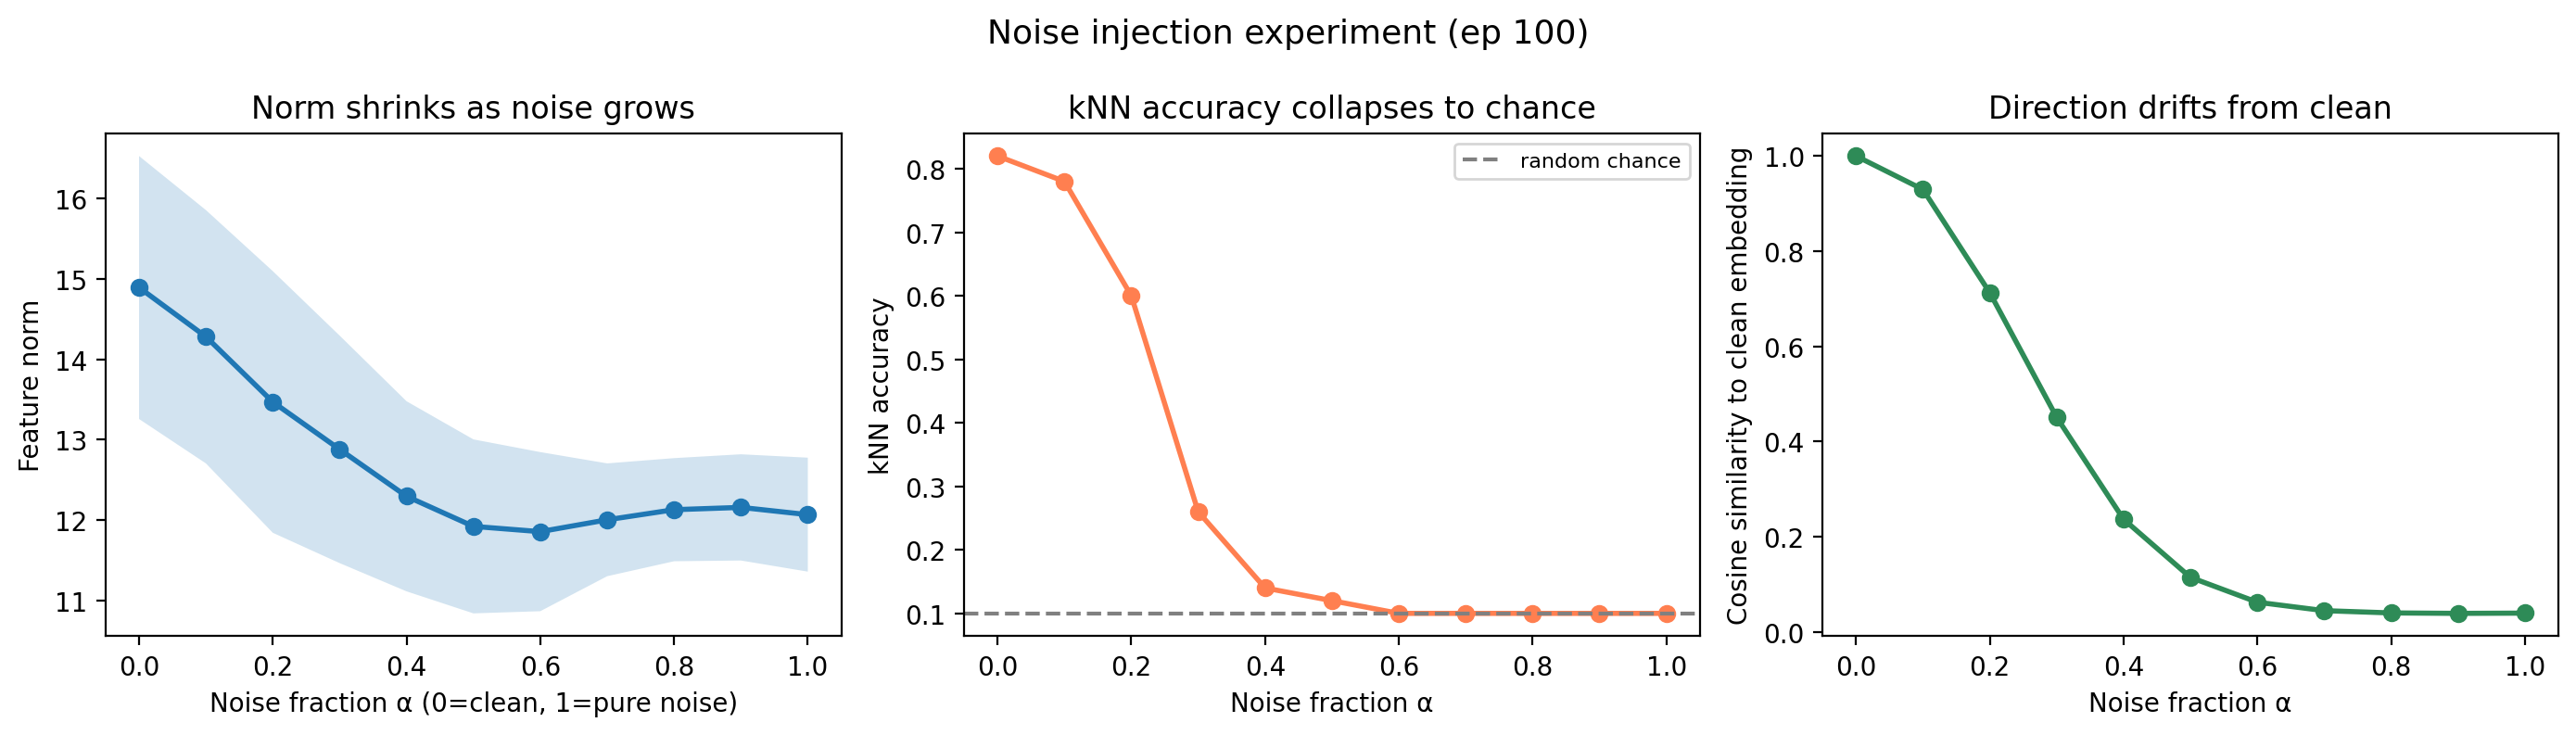
\includegraphics[width=\linewidth]{figures/noise_summary_ep100.png}
    \caption{Noise-mixing response of the flat-Gaussian SSL encoder. Left: feature norm decreases from $14.8$ at $\alpha = 0$ to a floor of $\sim 11.5$ at $\alpha \approx 0.5$, with a slight uptick back to $\sim 12$ at pure noise. Middle: $k$-NN accuracy collapses to chance by $\alpha \approx 0.5$. Right: cosine similarity to the clean embedding decays smoothly. Shaded regions are per-sample standard deviations.}
    \label{fig:noise_summary}
\end{figure}

Mean feature norm drops from $14.89$ at $\alpha = 0$ to $11.92$ at $\alpha = 0.5$ and plateaus near $11.9$--$12.2$ for $\alpha \ge 0.5$, with a small \emph{increase} from $\alpha = 0.6$ to $\alpha = 1.0$ discussed below. Simultaneously, $k$-NN accuracy on this subset collapses from $82\%$ at $\alpha = 0$ to $12\%$ (approaching chance) by $\alpha = 0.5$ (note: the clean accuracy is on a $100$-sample stratified subset; the full-validation-set clean accuracy is $75\%$). The cosine similarity between the noisy and clean embeddings decays smoothly from $1$ to near zero, indicating that the direction of the feature also drifts, but more gradually than the norm collapses.

\paragraph{A stable ``noise manifold''.} The fact that the feature norm does not continue to fall as $\alpha \to 1$---and in fact rises slightly---is notable. Different noise samples all produce features of similar norm $\sim 12.1$, suggesting that pure-noise inputs are mapped to a consistent region of embedding space rather than to arbitrary locations. We characterize this region directly in \secref{sec:noise_subspace}.

\subsection{The Noise Subspace}
\label{sec:noise_subspace}

We embed $2{,}000$ real CIFAR-10 validation images and $500$ independent pure-noise images through the same encoder, and compare the two feature sets.

\paragraph{Effective dimensionality.} We measure effective dimensionality as $\exp\!\left(-\sum_i p_i \log p_i\right)$, where $p_i$ is the $i$-th entry of the normalized PCA spectrum. For the real-image features this is $\approx 237$ of $256$; for noise features it is $\approx 12$. Pure noise collapses into roughly $5\%$ of the ambient dimensionality (\figref{fig:noise_subspace_pca}, top).

\paragraph{Angular relationship to classes.} Let $\bar{\vect{z}}_c$ denote the mean feature of class $c$ in the real-image set and $\bar{\vect{z}}_\text{noise}$ the mean noise feature. The angle between $\bar{\vect{z}}_\text{noise}$ and each class mean ranges from $66^\circ$ (\texttt{frog}) to $82^\circ$ (\texttt{ship}); the mean angle between distinct class means is $63^\circ$. Noise is, in angular terms, \emph{further} from every class than classes are from each other---it occupies a direction that is roughly orthogonal to the class manifold.

\paragraph{UMAP.} \figref{fig:noise_subspace_pca} (bottom) shows a UMAP \citep{mcinnes2018umap} embedding of the real-image and noise features. The two sets are completely disjoint in the projection: noise forms a tight cluster that does not overlap any class region.

\begin{figure}[t]
    \centering
    \begin{subfigure}{\linewidth}
        \centering
        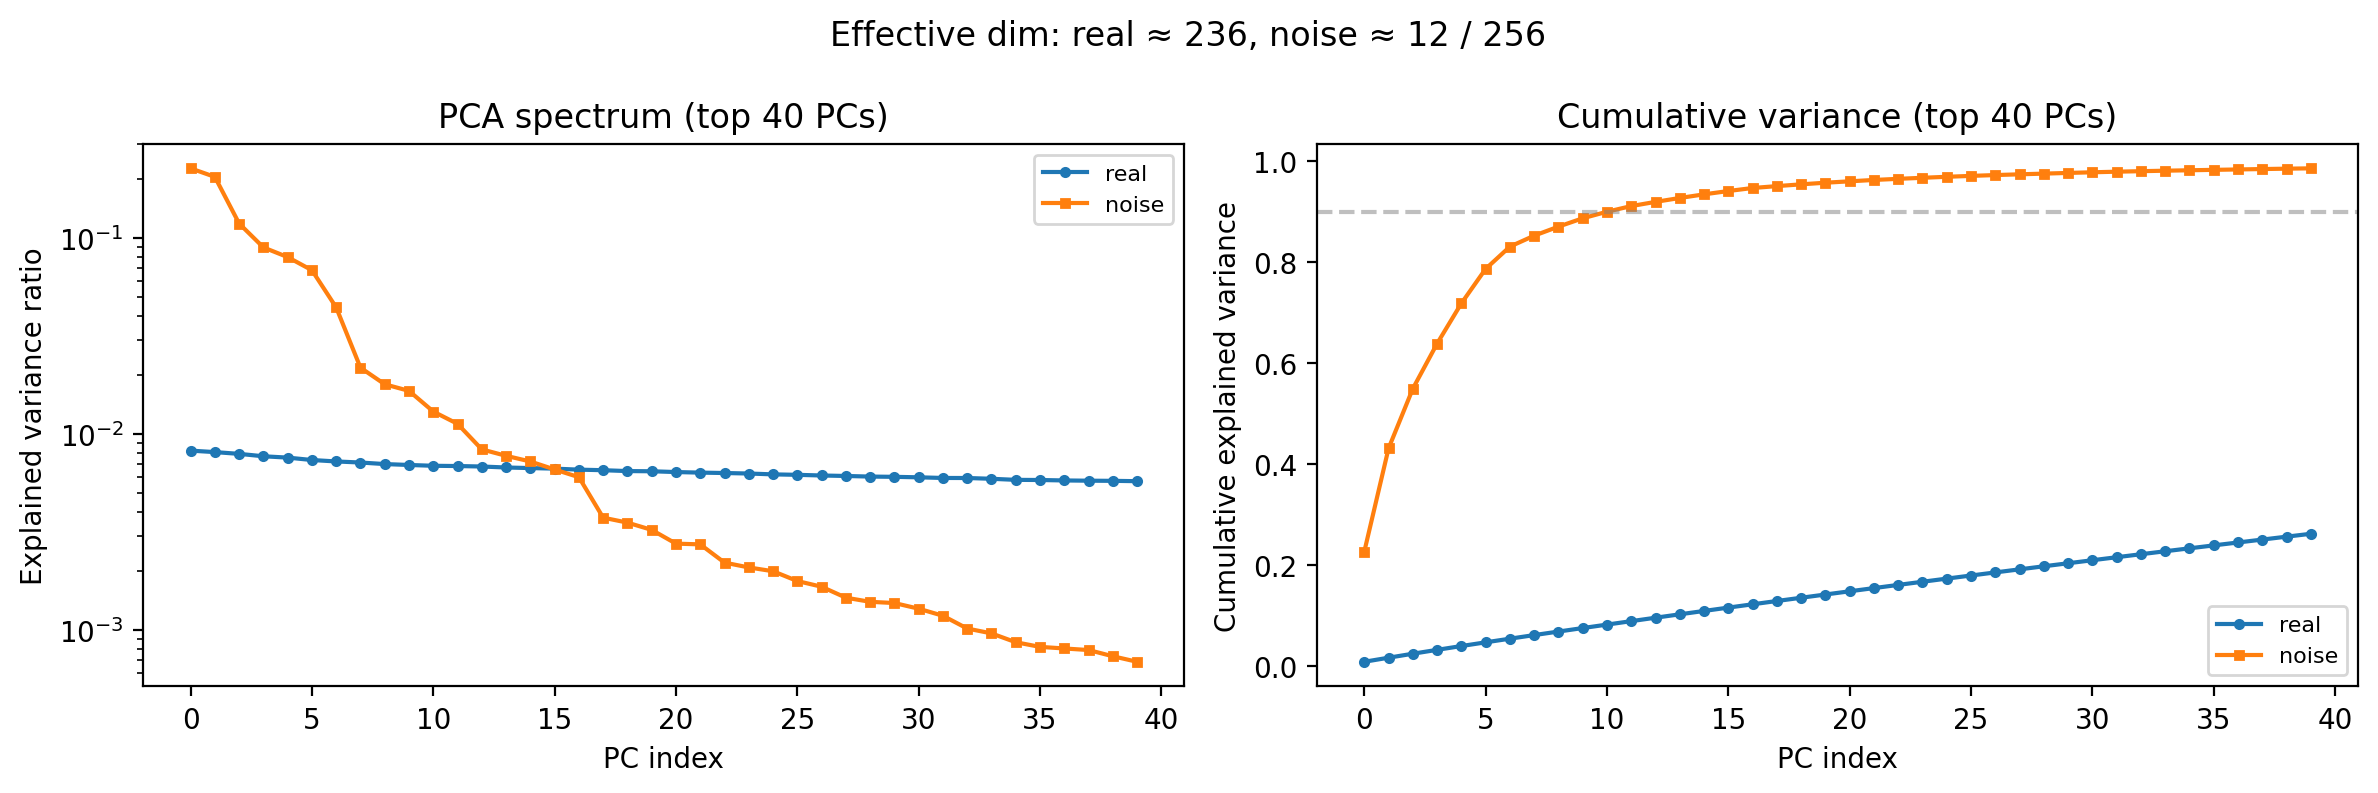
\includegraphics[width=0.9\linewidth]{figures/noise_subspace_pca_ep100.png}
    \end{subfigure}\\[3pt]
    \begin{subfigure}{\linewidth}
        \centering
        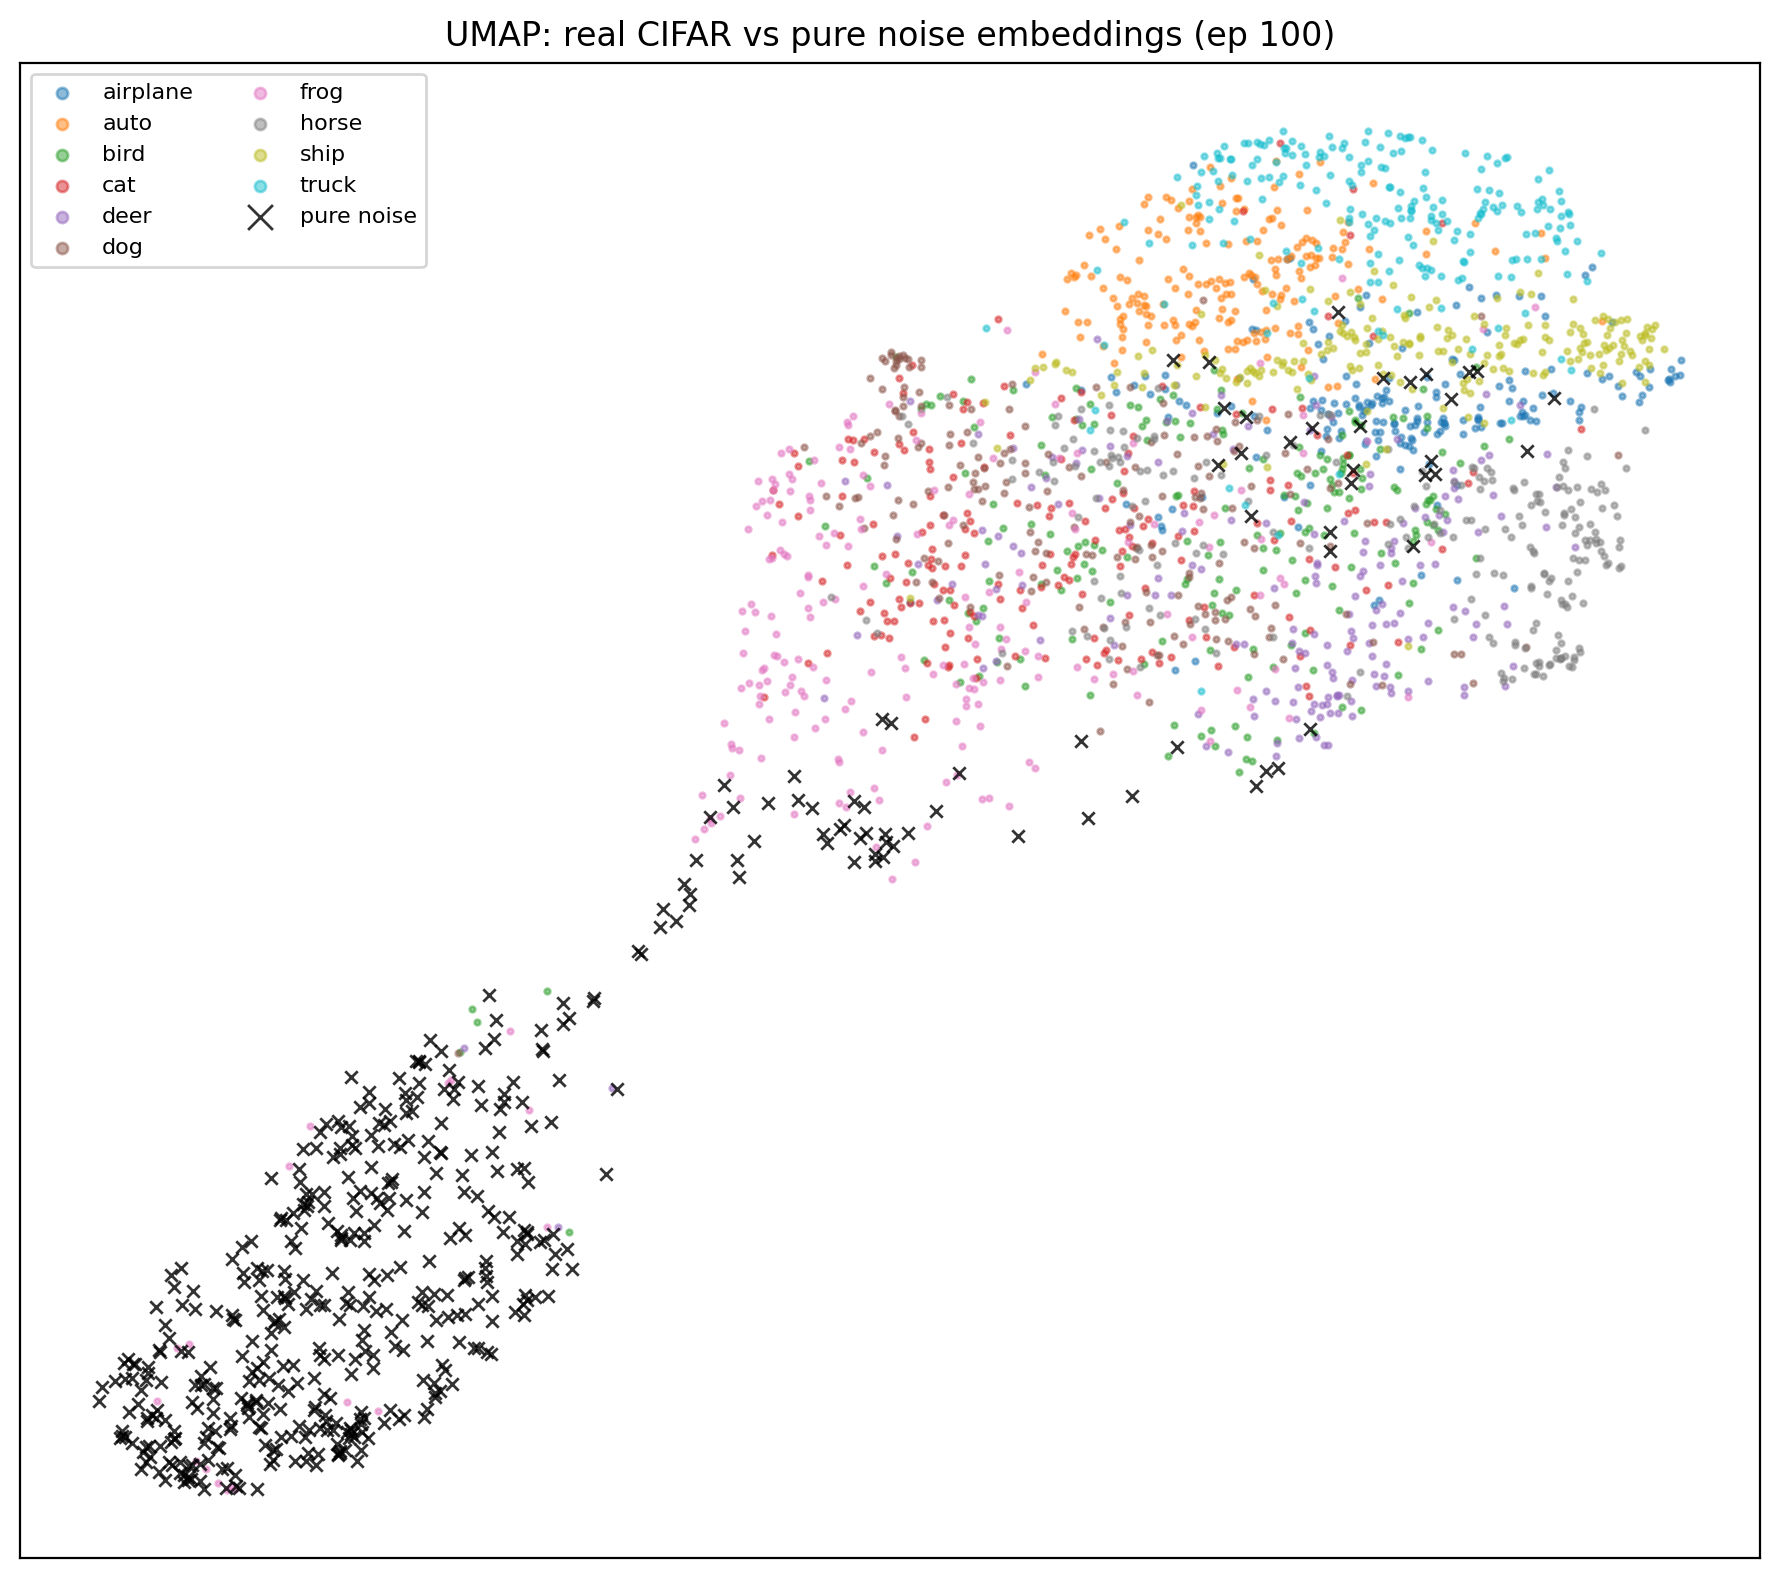
\includegraphics[width=0.55\linewidth]{figures/noise_subspace_umap_ep100.png}
    \end{subfigure}
    \caption{Top: PCA spectrum of real (flat) vs noise (steep) features; effective dimensions are $237$ and $12$ respectively. Bottom: UMAP embedding of the combined feature set. Noise samples ($\times$) form a cluster completely disjoint from the real-image classes.}
    \label{fig:noise_subspace_pca}
\end{figure}

\subsection{Comparison with DINOv2}
\label{sec:dinov2}

The behaviour documented above could be a generic property of joint-embedding SSL, or it could be specific to the flat-Gaussian geometry. To distinguish these, we repeat the noise-mixing experiment on a pretrained DINOv2 ViT-S/14 model \citep{oquab2023dinov2}, using the (unnormalized) CLS token and the mean-pooled patch tokens from \texttt{forward\_features}. CIFAR-10 inputs are bilinearly upsampled from $32 \times 32$ to $224 \times 224$ to match DINOv2's expected resolution. The same noise-mixing protocol applies.

\begin{figure}[t]
    \centering
    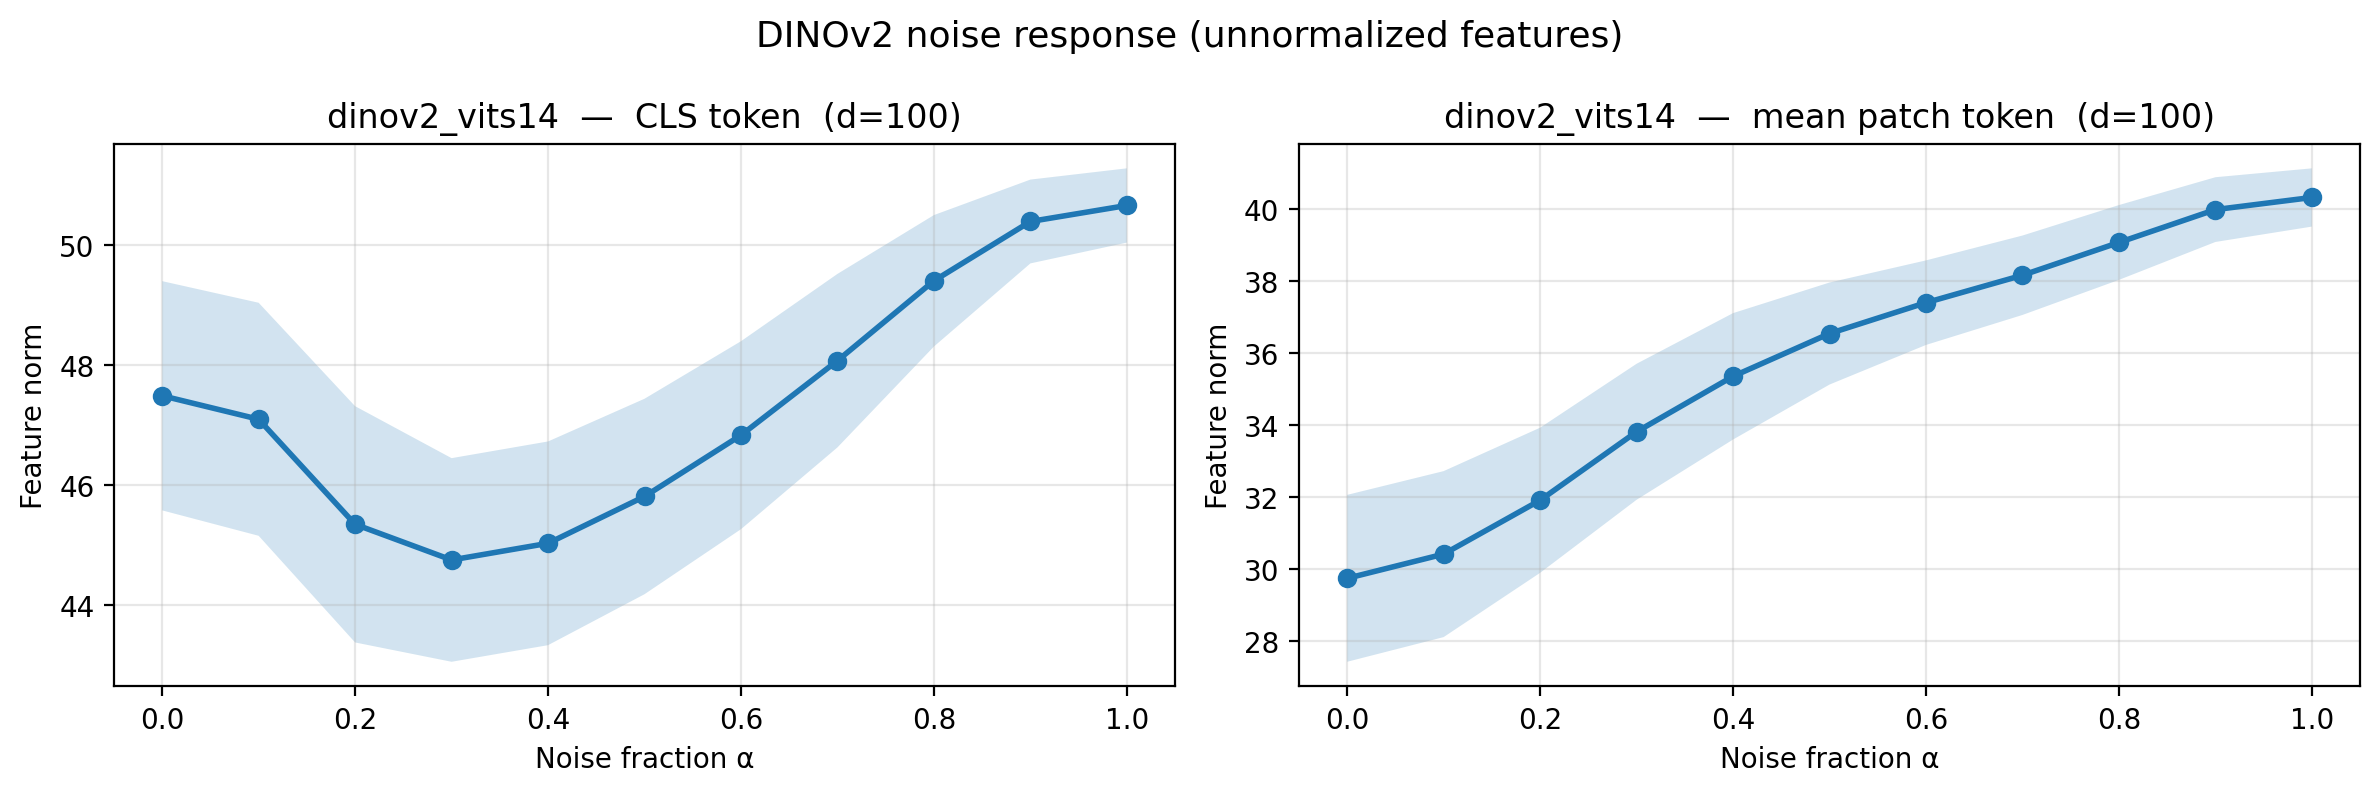
\includegraphics[width=\linewidth]{figures/noise_dinov2_dinov2_vits14.png}
    \caption{DINOv2 ViT-S/14 noise response. Left: CLS token norm has a shallow dip at $\alpha \approx 0.3$ and then \emph{rises} past the clean value, reaching a maximum at $\alpha = 1$. Right: mean-pooled patch-token norm rises \emph{monotonically} with noise fraction. In contrast to \figref{fig:noise_summary}, pure noise produces the highest-norm features.}
    \label{fig:noise_dinov2}
\end{figure}

\figref{fig:noise_dinov2} shows the result. Both of DINOv2's backbone features behave very differently from our flat-space features:
\begin{itemize}
    \item The CLS-token norm has a shallow V-shape, dipping from $47.5$ (clean) to $44.8$ at $\alpha = 0.3$, then \emph{rising} back above clean to $50.7$ at pure noise. There is no monotone relationship between noise fraction and feature norm.
    \item The mean patch-token norm rises \emph{monotonically} with noise from $29.8$ (clean) to $40.3$ (pure noise). Higher norm corresponds to \emph{lower} confidence.
\end{itemize}

Whatever mechanism causes noise inputs in our flat-Gaussian model to migrate toward the origin and occupy a low-dimensional subspace is not a generic property of self-supervised ViTs. DINOv2, trained with a cross-entropy-over-prototypes objective on normalized features, does not learn such a structure; if anything, its feature norm anti-correlates with confidence.

\paragraph{Caveat.} CIFAR inputs upsampled to $224 \times 224$ are mildly out-of-distribution for DINOv2 (trained on ImageNet at native resolution). The pattern warrants re-testing on native ImageNet validation images; preliminary runs (not shown) show the same qualitative direction, but a more careful comparison is future work.

\subsection{Summary of Findings}

We have shown, for a ResNet-18 trained on CIFAR-10 with a minimal flat-Gaussian SSL objective:
\begin{enumerate}
    \item the feature norm is strongly correlated with $k$-NN accuracy, with high-norm samples classified at $\approx 2\times$ the accuracy of low-norm samples;
    \item the norm is almost perfectly correlated ($r = 0.99$) with distance from the class centroid in feature space;
    \item adding uniform noise to the input radially contracts the embedding toward a stable low-norm region;
    \item pure-noise inputs collapse into a $\sim 13$-dimensional subspace, oriented roughly orthogonal to every class direction;
    \item none of the above is present in the publicly available DINOv2 model; if anything, the sign of the relationship is reversed.
\end{enumerate}

The combination suggests that feature norm in flat-Gaussian SSL encodes something close to a confidence or canonicalness score, without any supervised signal to that effect. We discuss interpretation and limitations in the next section.


\FloatBarrier
\bibliographystyle{plainnat}
\bibliography{references}

\end{document}
